\documentclass{standalone}
\usepackage{tikz}
\usetikzlibrary{patterns}
\usetikzlibrary{positioning}
\usetikzlibrary{patterns, positioning}
\usetikzlibrary{shapes.misc}
\usepackage[outline]{contour}
\contourlength{1.5pt} 
\usepackage[sfdefault]{ClearSans}

\begin{document}
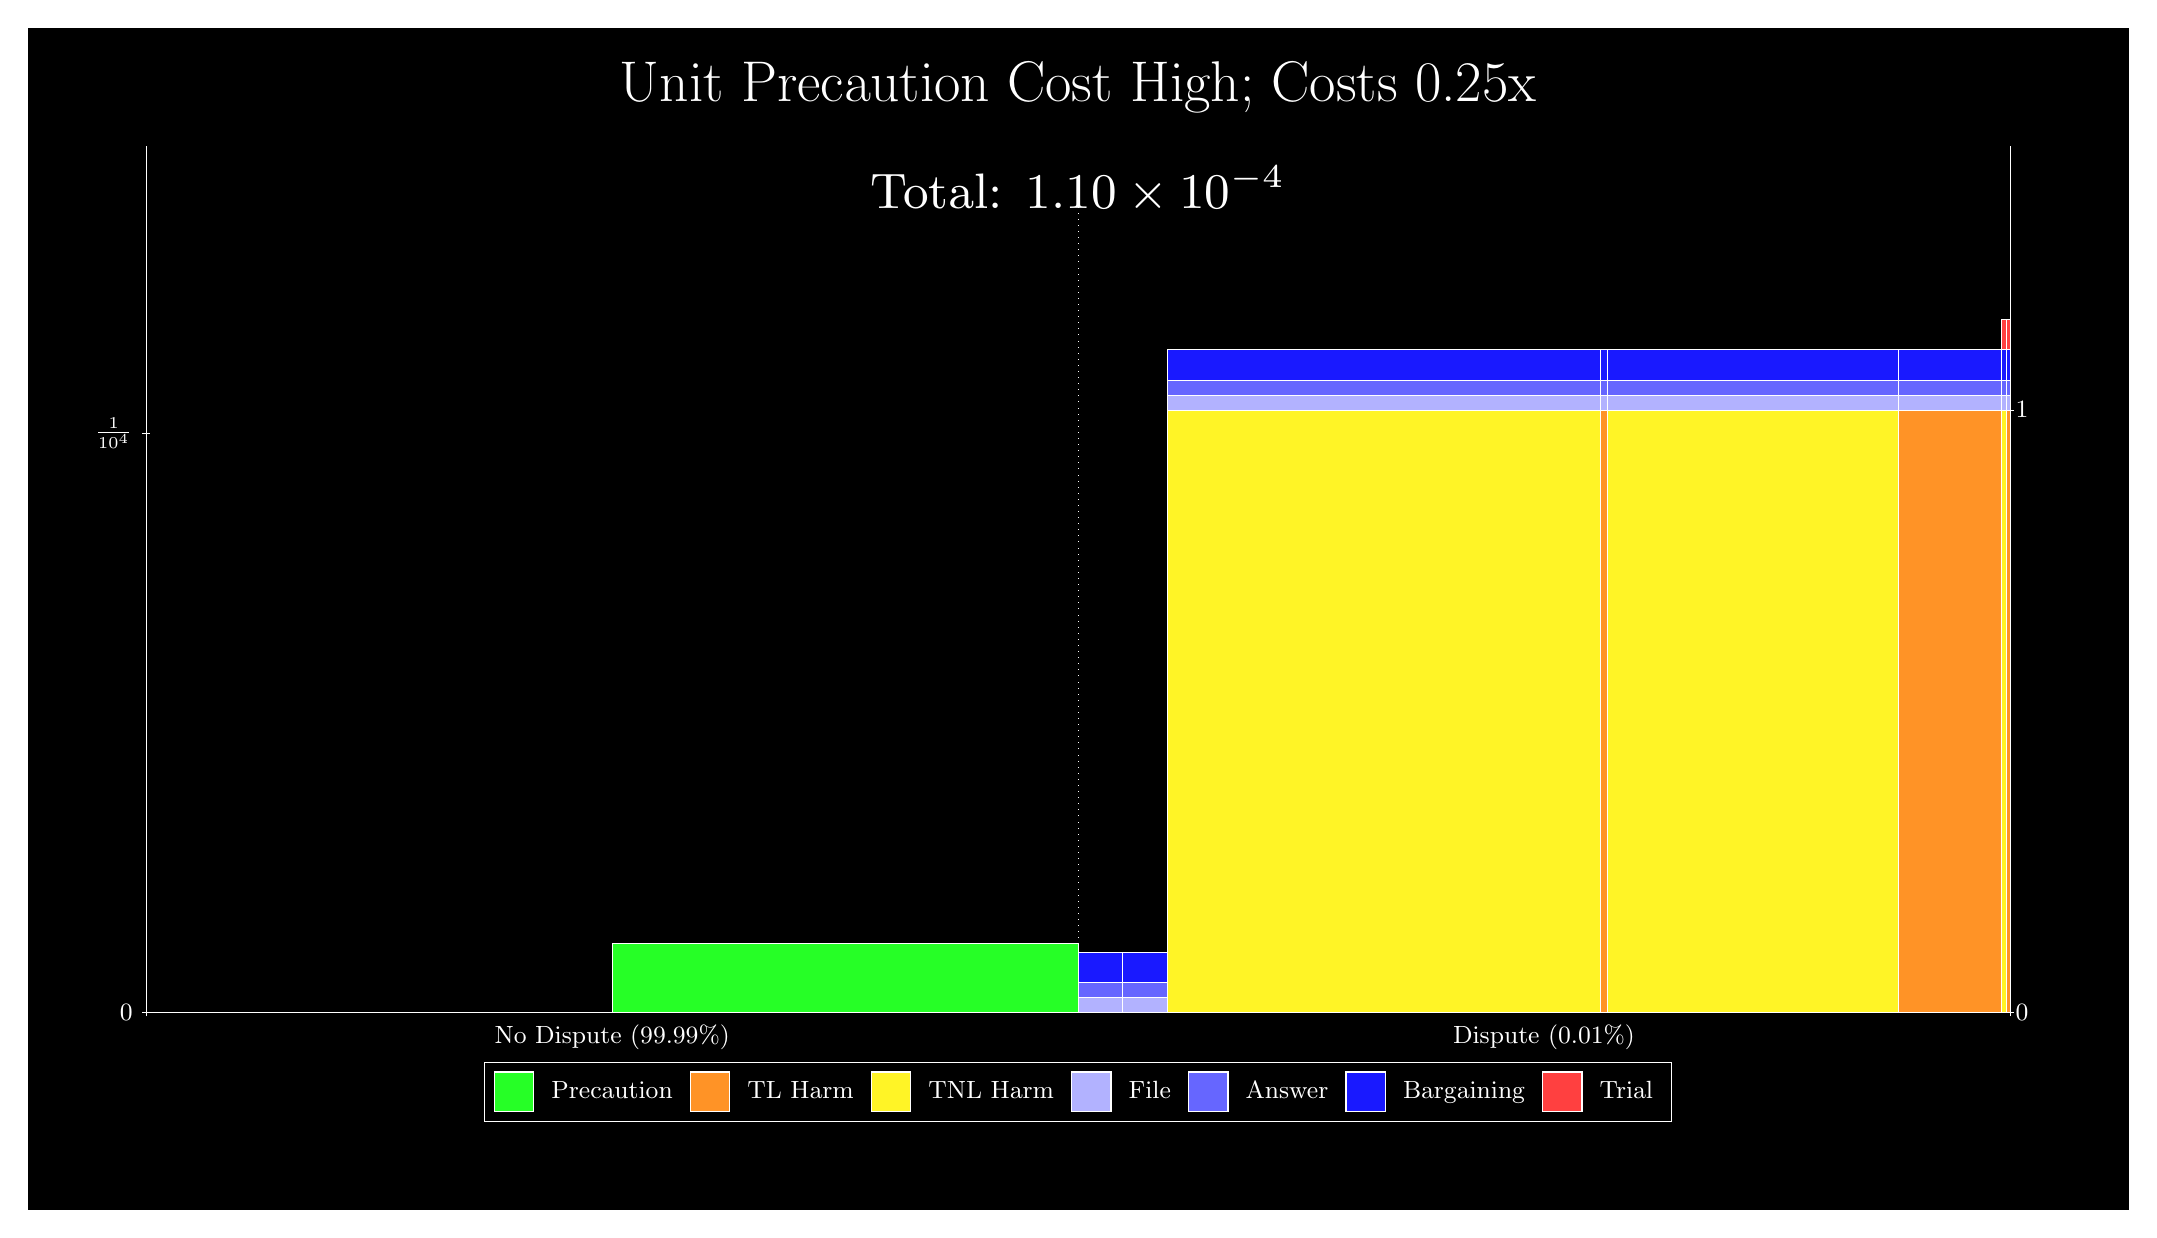
\begin{tikzpicture}
\draw[fill=black] (0,0) rectangle (26.667,15);
\draw[draw=none,text=white] (0,13.5) rectangle (26.667,15) node[midway] {\huge Unit Precaution Cost High; Costs 0.25x};
\draw[fill=green!85,draw=white,very thin] (7.4166,2.5) rectangle (13.333,3.3829);
\draw[fill=blue!30,draw=white,very thin] (13.333,2.5) rectangle (13.891,2.6913);
\draw[fill=blue!60,draw=white,very thin] (13.333,2.6913) rectangle (13.891,2.8826);
\draw[fill=blue!90,draw=white,very thin] (13.333,2.8826) rectangle (13.891,3.2652);
\draw[fill=green!85,draw=white,very thin] (13.891,2.5) rectangle (14.461,2.5001);
\draw[fill=blue!30,draw=white,very thin] (13.891,2.5001) rectangle (14.461,2.6914);
\draw[fill=blue!60,draw=white,very thin] (13.891,2.6914) rectangle (14.461,2.8827);
\draw[fill=blue!90,draw=white,very thin] (13.891,2.8827) rectangle (14.461,3.2653);
\draw[fill=blue!30,draw=white,very thin] (14.461,2.5) rectangle (14.471,2.6913);
\draw[fill=blue!60,draw=white,very thin] (14.461,2.6913) rectangle (14.471,2.8826);
\draw[fill=blue!90,draw=white,very thin] (14.461,2.8826) rectangle (14.471,3.2652);
\draw[fill=red!75,draw=white,very thin] (14.461,3.2652) rectangle (14.471,3.6478);
\draw[fill=yellow!85,draw=white,very thin] (14.471,2.5) rectangle (19.967,10.152);
\draw[fill=blue!30,draw=white,very thin] (14.471,10.152) rectangle (19.967,10.343);
\draw[fill=blue!60,draw=white,very thin] (14.471,10.343) rectangle (19.967,10.535);
\draw[fill=blue!90,draw=white,very thin] (14.471,10.535) rectangle (19.967,10.917);
\draw[fill=orange!85,draw=white,very thin] (19.967,2.5) rectangle (20.052,10.152);
\draw[fill=blue!30,draw=white,very thin] (19.967,10.152) rectangle (20.052,10.343);
\draw[fill=blue!60,draw=white,very thin] (19.967,10.343) rectangle (20.052,10.535);
\draw[fill=blue!90,draw=white,very thin] (19.967,10.535) rectangle (20.052,10.917);
\draw[fill=green!85,draw=white,very thin] (20.052,2.5) rectangle (23.747,2.5001);
\draw[fill=yellow!85,draw=white,very thin] (20.052,2.5001) rectangle (23.747,10.152);
\draw[fill=blue!30,draw=white,very thin] (20.052,10.152) rectangle (23.747,10.344);
\draw[fill=blue!60,draw=white,very thin] (20.052,10.344) rectangle (23.747,10.535);
\draw[fill=blue!90,draw=white,very thin] (20.052,10.535) rectangle (23.747,10.917);
\draw[fill=green!85,draw=white,very thin] (23.747,2.5) rectangle (25.058,2.5001);
\draw[fill=orange!85,draw=white,very thin] (23.747,2.5001) rectangle (25.058,10.152);
\draw[fill=blue!30,draw=white,very thin] (23.747,10.152) rectangle (25.058,10.344);
\draw[fill=blue!60,draw=white,very thin] (23.747,10.344) rectangle (25.058,10.535);
\draw[fill=blue!90,draw=white,very thin] (23.747,10.535) rectangle (25.058,10.917);
\draw[fill=yellow!85,draw=white,very thin] (25.058,2.5) rectangle (25.126,10.152);
\draw[fill=blue!30,draw=white,very thin] (25.058,10.152) rectangle (25.126,10.343);
\draw[fill=blue!60,draw=white,very thin] (25.058,10.343) rectangle (25.126,10.535);
\draw[fill=blue!90,draw=white,very thin] (25.058,10.535) rectangle (25.126,10.917);
\draw[fill=red!75,draw=white,very thin] (25.058,10.917) rectangle (25.126,11.3);
\draw[fill=orange!85,draw=white,very thin] (25.126,2.5) rectangle (25.167,10.152);
\draw[fill=blue!30,draw=white,very thin] (25.126,10.152) rectangle (25.167,10.343);
\draw[fill=blue!60,draw=white,very thin] (25.126,10.343) rectangle (25.167,10.535);
\draw[fill=blue!90,draw=white,very thin] (25.126,10.535) rectangle (25.167,10.917);
\draw[fill=red!75,draw=white,very thin] (25.126,10.917) rectangle (25.167,11.3);
\node[font=\small,text=white,anchor=north,scale=2] at (13.333, 13.5) {Total: $1.10\times 10^{-4}$};
\draw[white,very thin] (1.5,2.5) -- (1.5,13.5);
\draw[white,very thin] (1.45,2.5) -- (1.55,2.5);
\node[font=\small,text=white, anchor=east] at (1.45, 2.5) {0};
\draw[white,very thin] (1.45,9.8572) -- (1.55,9.8572);
\node[font=\small,text=white, anchor=east] at (1.45, 9.8572) {$\frac{1}{10^{4}}$};

\draw[white,dotted,very thin] (13.333,2.83) -- (13.333,13.17);
\draw[white,very thin] (25.167,2.5) -- (25.167,13.5);
\draw[white,very thin] (25.117,2.5) -- (25.217,2.5);
\node[font=\small,text=white, anchor=west] at (25.117, 2.5) {0};
\draw[white,very thin] (25.117,10.152) -- (25.217,10.152);
\node[font=\small,text=white, anchor=west] at (25.117, 10.152) {1};

\draw[white,very thin] (1.5,2.5) -- (25.167,2.5);
\draw[white,very thin] (1.5,2.45) -- (1.5,2.55);
\node[font=\small,text=white, anchor=north] at (1.5, 2.45) {};
\draw[white,very thin] (25.167,2.45) -- (25.167,2.55);
\node[font=\small,text=white, anchor=north] at (25.167, 2.45) {};

\node[font=\small,text=white,anchor=south] at (7.4167, 1.9) {No\ Dispute\ (99.99\%)};
\node[font=\small,text=white,anchor=south] at (19.25, 1.9) {Dispute\ (0.01\%)};
\draw (13.3333,2.5) node (B) {};
\begin{scope}[align=center]
\matrix[scale=0.5,draw=white,below=0.5cm of B,nodes={draw},column sep=0.1cm]{
\node[rectangle,draw,minimum width=0.5cm,minimum height=0.5cm,fill=green!85]{}; & \node[draw=none,font=\small,text=white]{Precaution}; &
\node[rectangle,draw,minimum width=0.5cm,minimum height=0.5cm,fill=orange!85]{}; & \node[draw=none,font=\small,text=white]{TL Harm}; &
\node[rectangle,draw,minimum width=0.5cm,minimum height=0.5cm,fill=yellow!85]{}; & \node[draw=none,font=\small,text=white]{TNL Harm}; &
\node[rectangle,draw,minimum width=0.5cm,minimum height=0.5cm,fill=blue!30]{}; & \node[draw=none,font=\small,text=white]{File}; &
\node[rectangle,draw,minimum width=0.5cm,minimum height=0.5cm,fill=blue!60]{}; & \node[draw=none,font=\small,text=white]{Answer}; &
\node[rectangle,draw,minimum width=0.5cm,minimum height=0.5cm,fill=blue!90]{}; & \node[draw=none,font=\small,text=white]{Bargaining}; &
\node[rectangle,draw,minimum width=0.5cm,minimum height=0.5cm,fill=red!75]{}; & \node[draw=none,font=\small,text=white]{Trial}; \\\\
};\end{scope}

\end{tikzpicture}
\end{document}